% NeurIPS 2026 Submission
\documentclass{article}
\usepackage[preprint]{neurips_approx}

\usepackage[utf8]{inputenc}
\usepackage[T1]{fontenc}
\usepackage{hyperref}
\usepackage{url}
\usepackage{booktabs}
\usepackage{amsfonts}
\usepackage{amsmath}
\usepackage{nicefrac}
\usepackage{microtype}
\usepackage{graphicx}
\graphicspath{{figures/}{diagrams/}}
\usepackage{xcolor}
\usepackage{algorithm}
\usepackage{algorithmic}
\usepackage{subcaption}
\usepackage{multirow}

\title{Can LLMs Improve at Debate Through Self-Play?\\A Pipeline and RL System to Gamify Competitive Debate\\with Branching and Hierarchical Rewards}

% Double-blind: anonymous submission
\author{Anonymous Authors}

\begin{document}

\maketitle

\begin{abstract}
Competitive debate is a demanding testbed for language model training: it
requires strategic planning, evidence integration, and adversarial reasoning
across many interdependent decisions. We present a training pipeline for
competitive AI debate in the International Public Debate Association (IPDA)
format, where each debate decomposes into ${\sim}33$ LLM calls spanning
planning, structuring, generation, and dialogue. Our system includes an
automated debate preparation pipeline that transforms a resolution into a
grounded debate via Bayesian belief-tree construction, a consolidated
research loop, and sentence-level-traceable evidence cards. On top of this
pipeline, we treat structured multi-turn debate generation as search: at each decision point we
produce and score multiple candidates, branching into parallel trajectories
when candidates diverge enough that opponent responses would differ. A
hierarchical reward system scores individual calls, backpropagates debate
outcomes to the specific decisions that caused them, and uses cross-branch
comparison to identify winner-shifting pivot points, feeding a group-wise
offline GRPO loop that trains heterogeneous call types as separate groups
with importance sampling.

In head-to-head tournament evaluation (68~debates on 17 held-out topics,
5-judge panel), the trained model wins 58.2\% of judge votes ($p = 0.034$,
GEE clustered on debate; Cohen's $d = 0.166$), with top tactics achieving
100\% success rates and group-wise GRPO reaching 81--88\% validation accuracy
across call types. We observe a structural side asymmetry (67.6\% negative
vs.\ 41.2\% affirmative, $p = 0.002$) present in the base model and amplified
by training, and document opposing LLM judge biases that partially cancel in
panel consensus. We release model checkpoints, training code, and a corpus
of 30+ judged debates with per-call scores.
\end{abstract}

\input{sections/01_introduction}
\section{Related Work}
\label{sec:related}

\paragraph{Computational Argumentation.}
Project Debater~\cite{slonim2021debater} demonstrated AI debate in a
simplified format designed for lay audiences, but explicitly acknowledged
its inability to engage in expert competitive debate. Prior work in
computational argumentation has focused on argument mining, stance detection,
and persuasion prediction rather than end-to-end debate generation, and
large-scale resources such as OpenDebateEvidence~\cite{roush2024opendebateevidence}
have primarily supported evidence retrieval and summarization rather than
trained debaters. We target the International Public Debate Association
(IPDA) format as an instance of competitive debate more broadly. Competitive
debate formats share typed argument structures
(Advantage = Uniqueness + Link + Impact~\cite{snider2008code}), explicit
rules, and specialist judges; we argue that these structured competitive
formats provide the discrete rewards needed for optimization.

\paragraph{Self-Play and Search in Games.}
Our branching mechanism draws on the tradition of self-play and tree search
in game-playing AI. AlphaGo Zero~\cite{silver2017mastering} and
AlphaZero~\cite{silver2018general} achieve superhuman performance via
Monte Carlo tree search (MCTS) guided by learned value and policy networks,
while OpenAI Five~\cite{berner2019dota} scaled self-play to the imperfect-information
setting of Dota~2. Unlike MCTS, which exhaustively explores game trees,
our branching is triggered only when candidate speeches would elicit
different opponent responses, focusing computation on informationally
rich divergence points. This threshold-based branching is closer to
selective search in that it expands only the nodes where counterfactual
outcomes are most likely to differ.

\paragraph{Tree Search with LLMs.}
Similar branching ideas appear in other RL-for-generation domains. Tree of
Thoughts~\cite{yao2023tree} expands reasoning trees at inference time using
self-evaluation heuristics, and RAP~\cite{hao2023reasoning} treats an LLM as
a world model and uses MCTS to search over reasoning steps guided by value
estimates. Our branching is related but operates on a different signal: we
branch based on \emph{opponent-response divergence} during adversarial
multi-agent rollouts rather than on self-consistency or value estimates, and
the resulting winner-shift events become training targets for offline GRPO
rather than an inference-time search procedure.

\paragraph{RL with Verifiable Rewards.}
Recent work on reasoning-oriented RL trains with programmatically verifiable
reward signals. DeepSeek-R1~\cite{guo2025deepseekr1} demonstrates that
large-scale RL with rule-based rewards elicits strong chain-of-thought
behaviors without supervised warm-start. Our three-layer reward hierarchy
occupies a middle ground: speech-level rubrics and branch-based winner-shift
detection provide near-verifiable local signals, while retrospective
multi-model panels handle the non-verifiable strategic quality of full
debates.

\paragraph{Debate as AI Alignment.}
Irving et al.~\cite{irving2018debate} proposed debate as a scalable oversight
mechanism, where competing agents help judges identify truthful answers.
Michael et al.~\cite{michael2023debate} showed that debate achieves 84\%
judge accuracy versus 74\% for consultancy, with debate errors decreasing
with debater skill. Du et al.~\cite{du2024multiagent} demonstrated that
multi-agent debate improves factuality through convergence dynamics. Our
work complements this line by studying the \emph{training dynamics} of
debate models rather than debate as an oversight protocol.

\paragraph{Constitutional AI and RLAIF.}
RLAIF~\cite{lee2024rlaif} replaces human annotators with LLM judges at
25--125$\times$ lower cost. Constitutional AI~\cite{bai2022constitutional}
showed that models can self-critique and revise outputs against a set of
principles, enabling alignment without human preference labels. Our
hierarchical reward system extends this idea: rather than a single
constitution, we employ speech-specific rubrics at Layer~1, causal outcome
attribution at Layer~2, and multi-model retrospective judging at Layer~3,
each providing a different form of AI-generated feedback.

\paragraph{Preference Optimization.}
We build on ORPO~\cite{hong2024orpo}, which eliminates
the reference model requirement of DPO~\cite{rafailov2023dpo}, and
offline GRPO~\cite{shao2024deepseekmath}, which uses importance sampling
ratios $\pi_\theta / \pi_{\text{ref}}$ to normalize for response
length---critical for tasks where quality does not correlate with verbosity.
Our contribution is the \emph{group-wise} application: decomposing
heterogeneous calls into four modality groups and training sequentially
with SFT-on-golden interleaving prevents the cross-modality interference
we observe when training all call types jointly.

\paragraph{LLM-as-Judge.}
LLM judges achieve 80\%+ human agreement but exhibit systematic
biases~\cite{zheng2023mtbench}: position bias, verbosity preference, and
self-enhancement. We document a novel bias pattern specific to adversarial
evaluation: different judge models exhibit \emph{opposing side biases}
(Section~\ref{sec:judge_bias}), motivating multi-model panels for debate
evaluation.

\section{Method}
\label{sec:method}

\subsection{IPDA Debate Format}

\begin{figure*}[t]
\centering
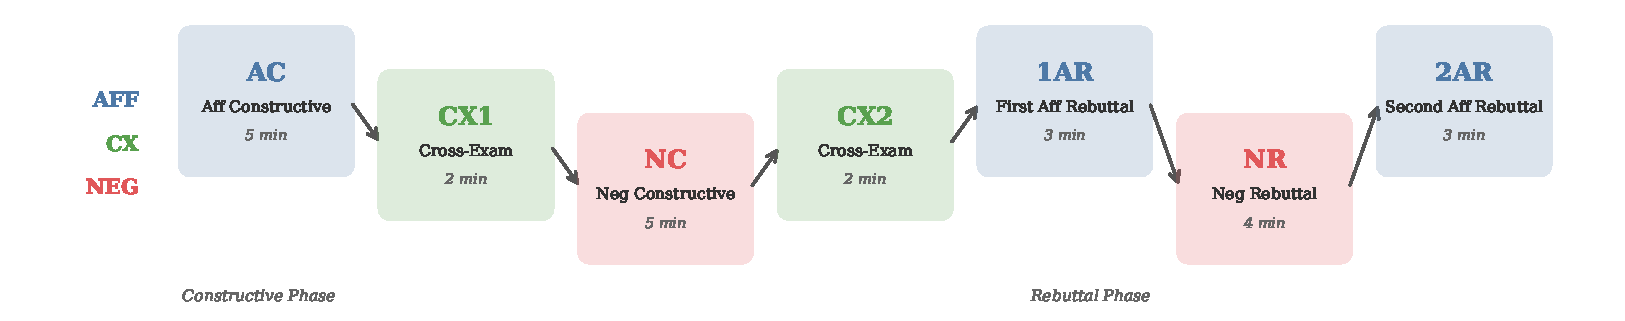
\includegraphics[width=\textwidth]{fig2_debate_sequence.pdf}
\caption{IPDA debate sequence: seven speeches alternating between
affirmative and negative with two cross-examination periods, each demanding
different capabilities (case generation, strategic response, dialogue).}
\label{fig:debate_sequence}
\end{figure*}

IPDA consists of 7 speeches alternating between affirmative and negative
(two constructives, two cross-examinations, three rebuttals;
Figure~\ref{fig:debate_sequence}). This structure is a natural curriculum:
constructives require case generation, rebuttals require strategic
response, and CX requires real-time dialogue, motivating our group-wise
training. Arguments follow typed syllogistic structures drawn from standard
debate theory~\cite{snider2008code}.

\subsection{Debate Generation Pipeline}
\label{sec:pipeline}

Before any training innovation can operate, the system must first produce
a complete, grounded debate from only a resolution. Our preparation
pipeline is the substrate on which branching, hierarchical reward, and
group-wise GRPO all operate, and it is shared identically between baseline
and experimental models, so downstream quality differences come from the
speech generation model, not from prep asymmetries.

\textbf{Belief tree.} A DSPy \textsc{ValueExtractor} produces 4
topic-specific values (2 per side); a \textsc{BeliefGenerator} expands
each to a depth-2 tree ($\sim$32 beliefs, $\sim$16 arguments per side).
Each belief carries a Bayesian credence in $[0,1]$, and arguments are
typed (uniqueness, link, impact, solvency, turn) for structured downstream
slots. \textbf{Research loop.} Per argument claim: LLM query generation
$\rightarrow$ parallel Weaviate$+$Tavily retrieval $\rightarrow$ sentence
chunking $\rightarrow$ hybrid scoring ($0.7\cdot\cos + 0.3\cdot$BM25)
$\rightarrow$ window expansion $\rightarrow$ structured LLM selection.
This consolidated loop uses \textbf{2 LLM calls per hop} vs.\ 9 in prior
systems, with most claims resolving in one hop. \textbf{Evidence cards}
store \texttt{full\_text}, \texttt{card} (with \textbf{bolded} selections),
\texttt{selected\_sentence\_ids}, and window ranges; speech generation
cites by sentence~ID only, so quotations are assembled verbatim and
fabrication is eliminated by construction. \textbf{Perspective building.}
A \textsc{PerspectiveBuilder} compiles side-specific prompts:
constructives get pruned depth-1 beliefs (2 of 4); rebuttals get the full
sub-belief tree in SEAM form (Setup, Evidence, Analysis, Move).
\textbf{Four-stage speech generation.} Each of the 7 speeches runs
(1)~\textsc{SelectTactic}, (2)~\textsc{BuildSkeleton},
(3)~\textsc{SelectEvidence} (constructives only; binds claims to
sentence~IDs), and (4)~\textsc{GenerateSpeech}. The training innovations
described next operate on calls produced by this pipeline. Full schemas
are in Appendix~\ref{app:pipeline}.

\subsection{Branching Debate Generation}
\label{sec:branching}

\begin{figure*}[t]
\centering
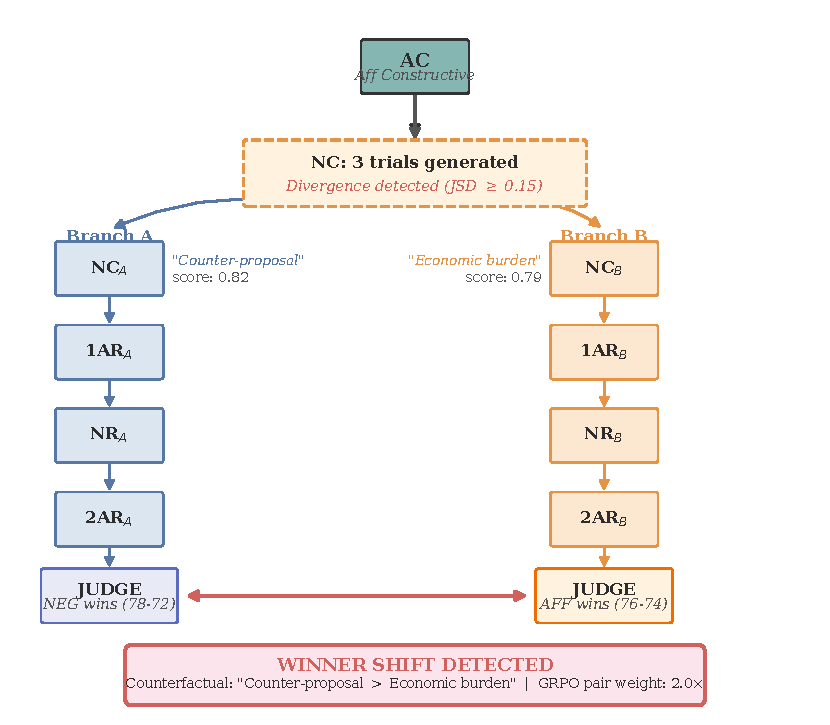
\includegraphics[width=\textwidth]{fig_branching_tree.pdf}
\caption{Branching debate tree. At each speech point, $N$ trials are
generated and scored; the debate forks when trials exceed quality
threshold and diverge enough that the opponent would respond differently.
Winner-shifts between branches yield counterfactual training pairs.}
\label{fig:branching_tree}
\end{figure*}

Standard debate generation is linear: produce one speech, continue to the
next. We instead treat debate generation as \textbf{search over debate
trajectories} (Figure~\ref{fig:branching_tree}). At each speech point, the model
generates $N = 3$ candidate trials scored by dimensional judges. When two
or more trials exceed a quality threshold \emph{and} diverge sufficiently
that the opponent would respond differently, the debate forks into parallel
paths (capped at 4 branches). The critical signal arises from
\textbf{winner-shift detection}: when branches from the same decision point
produce different debate outcomes, we obtain counterfactual training pairs
that receive $2\times$ weight in GRPO (Section~\ref{sec:grpo}), isolating
the specific decision that changed the result. Before each speech, the model
selects a named tactic via an epsilon-greedy policy, serving as a commitment
device that improves coherence. Full branching thresholds and the state
tracking algorithm are detailed in Appendix~\ref{app:branching}.

\subsection{Hierarchical Reward System}
\label{sec:reward_hierarchy}

\begin{figure*}[t]
\centering
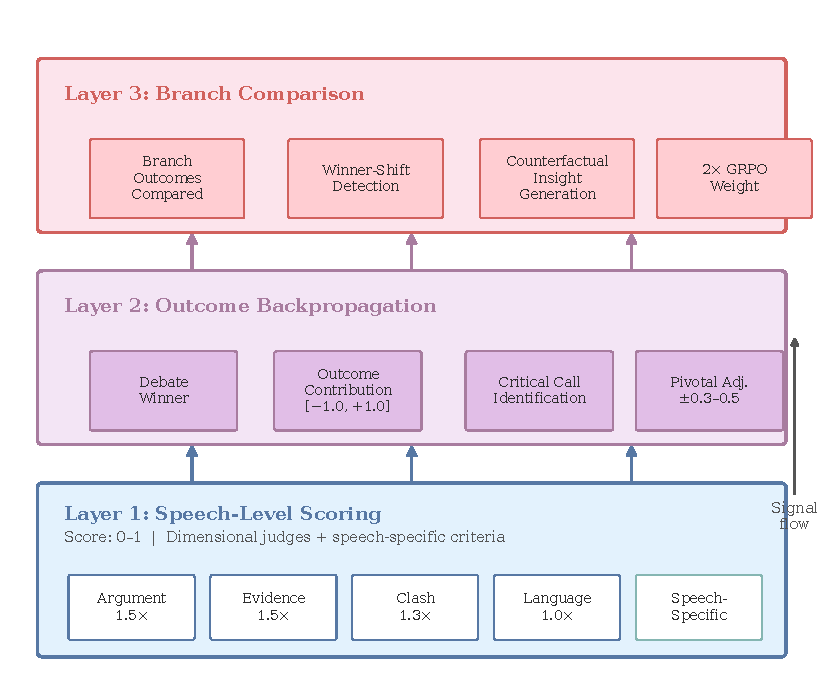
\includegraphics[width=\textwidth]{fig_reward_hierarchy.pdf}
\caption{Three-layer hierarchical reward. Layer~1: dimensional speech
scoring. Layer~2: outcome backpropagation to calls. Layer~3: multi-model
retrospective analysis for bias and turning points.}
\label{fig:reward_hierarchy}
\end{figure*}

Scoring isolated speeches is insufficient: a sound rebuttal can still lose
if it addresses the wrong arguments. We employ a three-layer reward
hierarchy (Figure~\ref{fig:reward_hierarchy}).

\paragraph{Layer 1: Dimensional scoring.}
Four sub-judges (ArgumentJudge, EvidenceJudge, ClashJudge, LanguageJudge)
score each speech with specialized rubrics, plus a speech-specific
dimension reflecting strategic role (e.g., 1AR \emph{triage efficiency},
2AR \emph{crystallization}; Appendix~\ref{app:agentic_judge}).

\paragraph{Layer 2: Outcome backpropagation.}
A BackpropScorer propagates debate outcomes to individual calls with
causal attribution, assigning each speech a contribution in $[-1.0, +1.0]$.
Winner-shift events from branching produce direct adjustments at the
divergence point, so a strong speech in a losing debate is not punished
if the loss originated earlier.

\paragraph{Layer 3: Meta-debate comparison.}
A 3-model retrospective panel evaluates complete traces, detecting bias
and identifying turning points that become highest-signal training data.

\paragraph{Evidence verification.}
Models cite by sentence ID, assembling verbatim text from research
documents---eliminating fabrication by construction. Evidence quality
uses a 6-level scale with $2\times$ asymmetric GRPO penalty on
fabrications.

\subsection{Group-Wise Offline GRPO}
\label{sec:grpo}

\begin{algorithm}[t]
\caption{Group-Wise Offline GRPO for Debate}
\label{alg:training}
\begin{algorithmic}[1]
\FOR{$i = 1$ to $N$ iterations}
    \STATE Generate debates with branching; capture log-probs
    \STATE Score with 3-layer reward hierarchy
    \FOR{group $\in \{A, B, C, D\}$}
        \STATE Generate Opus golden samples for group
        \STATE SFT on golden $\rightarrow$ merge to SFT$^+$
        \STATE Generate new trials with SFT$^+$; capture log-probs
        \STATE Offline GRPO with importance sampling
        \STATE Merge LoRA $\rightarrow$ canonical model
    \ENDFOR
\ENDFOR
\end{algorithmic}
\end{algorithm}

A debate produces $\sim$33 LLM calls spanning radically different output
modalities: $\sim$200-token tactic selections, $\sim$2{,}000-token
speeches, and multi-turn CX. Training jointly creates noisy gradients as
the optimizer tries to satisfy contradictory length and format
distributions. We \textbf{decompose calls into four groups} processed
sequentially each iteration (Algorithm~\ref{alg:training}):

\begin{table}[t]
\centering
\small
\begin{tabular}{llcc}
\toprule
\textbf{Group} & \textbf{Call Types} & \textbf{Samples} & \textbf{Output Length} \\
\midrule
A & \textsc{tactic\_select} & $\sim$3K & Short \\
B & \textsc{skeleton\_build}, \textsc{evidence\_select} & $\sim$4K & Medium \\
C & \textsc{speech\_generate} & $\sim$4.5K & Long \\
D & \textsc{cx\_dialogue} & $\sim$5K & Dialogue \\
\bottomrule
\end{tabular}
\caption{Call-type groups for sequential GRPO training. Each group contains
calls with similar output modality and length distribution, preventing
cross-modality gradient interference.}
\label{tab:call_types}
\end{table}

For each group, we: (1)~generate Opus golden samples as quality upper
bounds, (2)~SFT on golden samples via LoRA ($r = 32$) to produce an SFT$^+$
checkpoint, (3)~generate new trials with SFT$^+$ while capturing
log-probabilities for the behavior policy, (4)~run offline
GRPO~\cite{shao2024deepseekmath} with importance sampling, and (5)~merge
the LoRA into the canonical model as baseline for the next group.
Advantages are normalized within \emph{(our\_tactic, opponent\_tactic,
opponent\_intent)} triplets rather than globally, yielding cleaner gradient
signal. Full details are in Appendix~\ref{app:grpo_groups}.

\paragraph{Judge design.}
Beyond the four Layer~1 sub-judges, a \textbf{Chronicler} tracks each
argument's status (standing, attacked, dropped, extended, conceded, turned)
across the debate, and a \textbf{Forensics module} attributes failures to
specific pipeline stages (tactic, skeleton, evidence, execution). For each
call, $N = 3$ trials at varied temperatures produce chosen/rejected
preference pairs, yielding $\sim$60+ pairs per debate
(Appendix~\ref{app:agentic_judge}).

\input{sections/04_experiments}
\input{sections/05_analysis}
\input{sections/06_conclusion}

\bibliographystyle{plain}
\bibliography{references}

\appendix
\section{Extended Method Details}
\label{app:method_details}

This appendix documents the implementation details of the training pipeline
referenced in Section~\ref{sec:method}: model configuration, the epsilon-greedy
tactic exploration policy, the full research pipeline used for evidence curation,
and the evidence verification rubric.

\subsection{Model Configuration}

\begin{table}[h]
\centering
\small
\begin{tabular}{ll}
\toprule
\textbf{Parameter} & \textbf{Value} \\
\midrule
Base model & Qwen3-30B-A3B-Thinking (MoE: 30B total, 3B active) \\
LoRA rank & 32, $\alpha$=64, targets: q/k/v/o projections \\
LoRA dropout & 0.05 \\
ORPO $\beta$ & 0.1 \\
Learning rate & $5 \times 10^{-7}$ \\
Epochs per iteration & 2 \\
DeepSpeed & ZeRO-3 across 8 GPUs \\
Inference & vLLM with tensor parallelism \\
\bottomrule
\end{tabular}
\caption{Training configuration for Phase~1 iterative ORPO.}
\label{tab:model_config}
\end{table}

\subsection{Epsilon-Greedy Tactic Exploration}

The tactical playbook uses a 3-tier hierarchy:
\begin{itemize}
    \item \textbf{AtomicActions} ($\sim$21K): Single debate moves (77 ActionTypes $\times$ 39 TargetTypes $\times$ 7 PrivateIntents)
    \item \textbf{MicroTactics} ($\sim$10$^9$): 2--4 move sequences, the GRPO optimization unit
    \item \textbf{MacroTactics} (25+): Named strategies with game-theoretic payoff matrices
\end{itemize}

Sampling uses epsilon-greedy: $\sim$70\% exploit (proven tactics), $\sim$25\% explore (novel combinations), $\sim$5\% innovate (random). Tactics are promoted to the permanent playbook when uses $\geq 5$ and avg\_reward $\geq 0.6$. Epsilon grows dynamically with playbook size: $\varepsilon = \min(0.9, \varepsilon_{\text{base}} + 0.003 \times \lfloor|\text{book}|/10\rfloor)$.

Speech-type-specific epsilon values: AC/NC (constructive) $\varepsilon = 0.6$--$0.7$; 1AR/NR (rebuttal) $\varepsilon = 0.4$; 2AR (final) $\varepsilon = 0.3$.

\subsection{Research Pipeline}

Evidence retrieval uses a consolidated pipeline:
\begin{enumerate}
    \item \textbf{LLM}: Generate search queries from debate context
    \item \textbf{Automated}: Search $\rightarrow$ clean (regex) $\rightarrow$ chunk (sentence-level) $\rightarrow$ score ($0.7 \times$ embedding $+ 0.3 \times$ BM25) $\rightarrow$ window expansion ($\pm$3 sentences)
    \item \textbf{LLM}: Select sentences by ID and format evidence cards
\end{enumerate}

This reduces the original 9-LLM-call pipeline to 2--3 calls per research hop ($\sim$\$0.05/hop, 10--15s latency).

\subsection{Evidence Verification Scoring}

Evidence quality uses a 6-level scale with asymmetric GRPO penalties:

\begin{table}[h]
\centering
\small
\begin{tabular}{lcc}
\toprule
\textbf{Category} & \textbf{Score} & \textbf{GRPO Weight} \\
\midrule
EXACT\_MATCH & +1.0 & 1.0$\times$ \\
PARAPHRASE & +0.7 & 1.0$\times$ \\
WEAK\_SUPPORT & +0.3 & 1.0$\times$ \\
MISQUOTE & $-$0.5 & 1.5$\times$ \\
FABRICATION & $-$0.8 & 2.0$\times$ \\
HALLUCINATION & $-$1.0 & 2.0$\times$ \\
\bottomrule
\end{tabular}
\caption{Evidence verification categories with asymmetric penalties.}
\end{table}

\subsection{Design Rationale}

\textbf{ORPO over DPO:} Iterative training requires no frozen reference model. DPO would require careful reference model scheduling across iterations.

\textbf{Trajectory-level evaluation:} Debate quality emerges from cumulative choices across speeches. Scoring complete debates captures strategic dynamics that per-turn evaluation misses.

\textbf{Sentence-ID selection over RAG:} Hard constraint prevents fabrication---invalid IDs fail at generation time, valid IDs guarantee verbatim text.

\input{appendix/appendix_b_experiment_details}
\section{Tournament Details}
\label{app:tournament_details}

This appendix provides the full tournament methodology and results for the
head-to-head evaluation referenced in Section~\ref{sec:tournament}: the
topic-selection procedure, per-topic outcomes, score distributions, full
statistical test battery, side-asymmetry and judge-bias visualizations,
and a comparison to an earlier tournament version.

\subsection{Topic Selection}
\label{app:topic_selection}

The 17 tournament resolutions were selected from a corpus of 54 candidate
topics through a judge-bias probe. For each candidate, we queried three
judge models (Claude Opus~4.5, Gemini~2.5~Pro, and GPT-5.2) with the
resolution and asked them to rate it on a 0--10 scale, where 0 indicates
complete support for the negative position, 5 indicates a neutral topic
with no directional preference, and 10 indicates complete support for the
affirmative. For each topic we computed the mean rating across judges and
the distance from 5.0; we selected the 17 topics with the smallest distance
as the tournament set.

A sample of selected topics with their bias distances:
\begin{itemize}
    \item ``The ends can justify the means'' (dist: 0.17)
    \item ``Mathematical objects exist independently of human minds'' (dist: 0.17)
    \item ``Deep learning will lead to artificial general intelligence'' (dist: 0.17)
    \item ``Moral truths are objective facts independent of human beliefs'' (dist: 0.30)
    \item ``Compulsory voting strengthens democracy'' (dist: 0.80)
\end{itemize}

This approach identifies topics where the chosen judge models express no
strong directional preference; it does not eliminate all sources of bias.
In particular, topics where judges are systematically wrong in the same
direction would appear unbiased by this metric but would still be biased
in absolute terms. The probing script is available at
\texttt{scripts/ipda\_experiment/iter3/tournament/probe\_topic\_bias.py}.

\subsection{Per-Topic Results}

\begin{table}[h]
\centering
\small
\begin{tabular}{p{6cm}ccr}
\toprule
\textbf{Topic} & \textbf{Wins} & \textbf{Win\%} & \textbf{Mean $\Delta$} \\
\midrule
\multicolumn{4}{l}{\textit{Strong topics ($\geq$75\% win rate)}} \\
Moral truths are objective facts & 3/4 & 75\% & $+10.0$ \\
Economic development causes democratization & 3/4 & 75\% & $+9.6$ \\
Remote work reduces productivity & 3/4 & 75\% & $+8.4$ \\
Direct instruction $>$ inquiry-based learning & 3/4 & 75\% & $+7.8$ \\
Compulsory voting strengthens democracy & 3/4 & 75\% & $+4.2$ \\
Economic sanctions are immoral & 3/4 & 75\% & $+3.0$ \\
Many-Worlds $>$ Copenhagen interpretation & 3/4 & 75\% & $+2.2$ \\
\midrule
\multicolumn{4}{l}{\textit{Split topics (50\% win rate)}} \\
The ends can justify the means & 2/4 & 50\% & $+11.5$ \\
Mathematical objects exist independently & 2/4 & 50\% & $+12.0$ \\
Voters capable of democratic accountability & 2/4 & 50\% & $+8.0$ \\
Language acquisition is primarily innate & 2/4 & 50\% & $+2.4$ \\
Eliminate teacher tenure & 2/4 & 50\% & $-1.6$ \\
UBI should replace means-tested welfare & 2/4 & 50\% & $-4.6$ \\
\midrule
\multicolumn{4}{l}{\textit{Weak topics ($\leq$25\% win rate)}} \\
Deep learning will lead to AGI & 1/4 & 25\% & $-4.1$ \\
Federal $>$ unitary government & 1/4 & 25\% & $-1.7$ \\
Saturated fat increases CVD risk & 1/4 & 25\% & $-13.5$ \\
International institutions constrain states & 1/4 & 25\% & $-7.4$ \\
\bottomrule
\end{tabular}
\caption{Per-topic tournament results (pipeline judge). The trained model excels on
abstract/philosophical topics but struggles on empirical/institutional topics.}
\end{table}

\subsection{Score Distribution}

\begin{figure}[h]
\centering
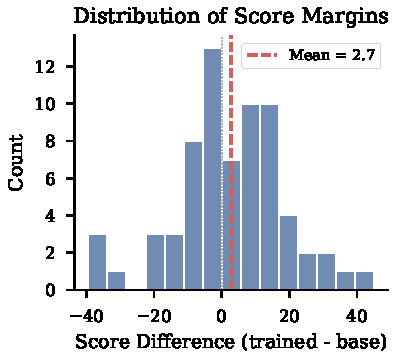
\includegraphics[width=\columnwidth]{fig_score_distribution.pdf}
\caption{Distribution of score differentials (trained $-$ base) across
68 debates. The distribution is right-skewed with mean $+2.7$, indicating
the trained model tends to win by larger margins than it loses.}
\label{fig:score_distribution}
\end{figure}

\begin{figure*}[h]
\centering
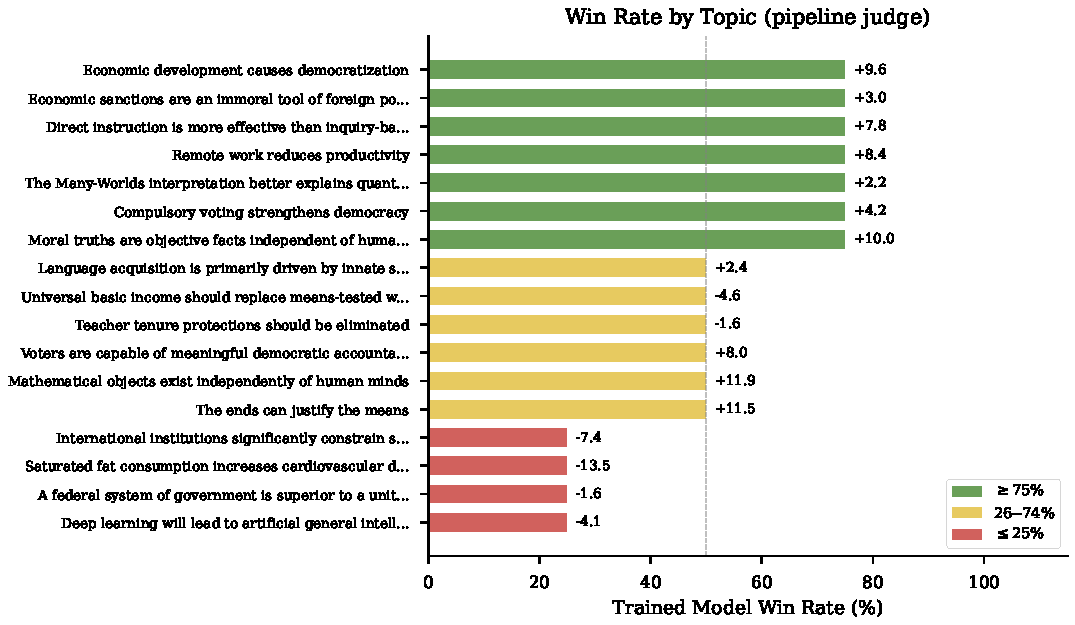
\includegraphics[width=\textwidth]{fig_topic_winrate.pdf}
\caption{Per-topic trained model win rate (pipeline judge, 4 debates per
topic). Green indicates $\geq$75\% win rate, yellow 50\%, red $\leq$25\%.
Annotations show mean score differential. The trained model dominates
abstract topics but struggles on evidence-dense empirical claims.}
\label{fig:topic_winrate}
\end{figure*}

Pipeline judge mean score difference: $+2.72$ (SD $= 16.38$).
The distribution is bimodal: the trained model wins decisively when it wins
(mean winning margin $+14.2$) but also loses decisively on certain
topic-side combinations (mean losing margin $-11.8$).

\begin{table}[h]
\centering
\begin{tabular}{lcc}
\toprule
\textbf{Score Diff Range} & \textbf{Count} & \textbf{\%} \\
\midrule
Trained $+10$+ & 22 & 32.4\% \\
Trained $+5$ to $+10$ & 8 & 11.8\% \\
Trained $+0$ to $+5$ & 7 & 10.3\% \\
Base $+0$ to $+5$ & 11 & 16.2\% \\
Base $+5$ to $+10$ & 10 & 14.7\% \\
Base $+10$+ & 10 & 14.7\% \\
\bottomrule
\end{tabular}
\caption{Score difference distribution (pipeline judge).}
\end{table}

\subsection{Statistical Tests}

\begin{table}[h]
\centering
\begin{tabular}{lcc}
\toprule
\textbf{Test} & \textbf{Statistic} & \textbf{$p$-value} \\
\midrule
Pipeline binomial (37/68) & -- & 0.545 \\
Panel binomial (38/68) & -- & 0.396 \\
Pooled binomial (198/340) & -- & 0.003 \\
Paired $t$-test (score diff) & $t(67) = 1.37$ & 0.175 \\
Wilcoxon signed-rank & $W = 909.5$ & 0.107 \\
Cohen's $d$ (pipeline) & 0.166 & -- \\
Side difference (Welch's $t$) & $t = 3.32$ & 0.002 \\
NEG wins binomial (23/34) & -- & 0.058 \\
AFF wins binomial (14/34) & -- & 0.392 \\
\bottomrule
\end{tabular}
\caption{Full statistical test battery for tournament results.}
\end{table}

\subsection{Side Asymmetry Visualization}

Figure~\ref{fig:side_asymmetry} visualizes the side-specific performance
reported in Table~\ref{tab:side_asymmetry}. The asymmetry holds whether
measured by win rate (41.2\% AFF vs.\ 67.6\% NEG), mean score differential
($-3.4$ AFF vs.\ $+8.9$ NEG), or Cohen's $d$ by side (0.09 AFF vs.\ 0.48 NEG).
Crucially, the base model also exhibits the same directional pattern (32.4\%
AFF vs.\ 58.8\% NEG from its own side perspective): the gap is structural
to IPDA, and training amplified rather than created it. We interpret this
as evidence that reactive argumentation (NEG, which speaks second and can
respond to concrete AFF claims) is more amenable to preference optimization
than generative argumentation (AFF, which must build a case from scratch).

\begin{figure}[h]
\centering
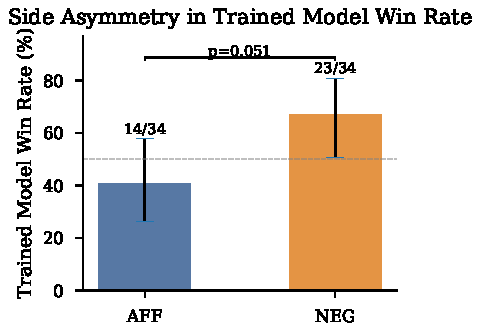
\includegraphics[width=\columnwidth]{fig_side_asymmetry.pdf}
\caption{Trained model win rate by debate side (pipeline judge, 68 debates).
The 26.4 percentage-point gap between affirmative (41.2\%) and negative
(67.6\%) win rates reflects a structural IPDA side advantage amplified
by training.}
\label{fig:side_asymmetry}
\end{figure}

\subsection{Judge Bias Analysis}

\begin{table}[h]
\centering
\small
\begin{tabular}{lcccc}
\toprule
\textbf{Judge} & \textbf{Trained\%} & \textbf{As AFF} & \textbf{As NEG} & \textbf{Retries} \\
\midrule
Gemini 2.5 & 54.4\% & 64.7\% & 44.1\% & 19\% \\
GPT-5.2 & 61.8\% & 29.4\% & 94.1\% & 22\% \\
Opus 4.5 & 60.3\% & 50.0\% & 70.6\% & 29\% \\
Sonnet 4 & 60.3\% & 32.4\% & 88.2\% & 43\% \\
\bottomrule
\end{tabular}
\caption{Per-judge voting patterns. GPT and Sonnet show extreme NEG-side
bias (94\%, 88\%); Gemini exhibits the opposite (65\% AFF). Opposing
biases partially cancel in panel consensus (55.9\%).}
\label{tab:judge_bias}
\end{table}

\begin{figure*}[h]
\centering
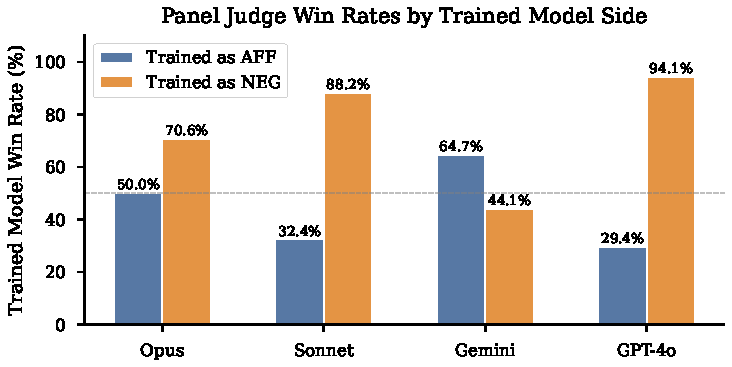
\includegraphics[width=\textwidth]{fig_judge_bias.pdf}
\caption{Per-judge voting patterns by trained model's debate side. GPT and
Sonnet show extreme NEG-side bias (94\%, 88\%), while Gemini exhibits the
opposite pattern (65\% AFF). Opus is the most balanced judge.}
\label{fig:judge_bias}
\end{figure*}

\subsection{Tournament V3 Comparison}

An earlier tournament (V3, 20 debates) showed no significant difference
(trained wins 9/20 = 45\%, $p = 0.82$). V3 had two infrastructure issues
that corrupted the signal: (i) panel judge API failures---Gemini and GPT
API keys were expired during parts of the run, leaving some debates scored
only by Claude judges, and (ii) 7 of the 20 debates had at least one
\texttt{null} speech due to generation timeouts, creating judge decisions
based on incomplete transcripts. V4 resolved both issues: all 68 debates
were generated to completion with retries on timeout, and all four panel
judges were healthy throughout the run. The 34-fold difference in
statistical power between V3 and V4 (20 vs.\ 340 judge-debate votes) is
the main reason V4 detects the effect that V3 missed; the underlying
trained-model advantage was present in both runs but only became
statistically distinguishable at V4's sample size.

\section{Failure Mode Analysis}
\label{app:failure_modes}

This appendix documents three failure modes encountered during training with
broader implications for RLAIF pipelines: the \emph{Bicameral Mind Problem}
(feedback hallucination in retry generation), the \emph{Retry Assumption
Failure} (inverted preference labels from unconditionally favoring retries),
and the \emph{Group~C Regression} (catastrophic divergence from full-LoRA
training on a Mixture-of-Experts base).

\subsection{The Bicameral Mind Problem}

During iteration~10, we discovered that 35.6\% of the model's thinking
sections contained hallucinated feedback---the model manufactured judge
criticism even when no prior feedback existed in the prompt.

\textbf{Quantification (644 samples):}
\begin{itemize}
    \item 226 contaminated samples from retry attempts
    \item Only 3 contaminated samples from first-attempt generations
    \item 28\% of ``chosen'' preference pairs referenced non-existent feedback
\end{itemize}

\textbf{Example (no feedback in prompt):}
\begin{quote}
\small
``We are now in a correction phase. The judge's feedback is severe: the
agent failed to conduct any searches...'' [No feedback was actually provided]
\end{quote}

\textbf{Root cause:} During training, retry attempts included judge feedback
in the conversation. The model learned to associate the debate task with
receiving criticism, hallucinating this pattern in fresh prompts---a form
of in-context learning contamination.

\textbf{Solution: Proactive self-coaching.} Replace reactive framing
(``the judge said you failed...'') with proactive framing (``when
approaching this task, I should verify every citation...'').
This prevents contamination because proactive thoughts don't require
imagining an external critic, and transfer cleanly to inference.

\textbf{General principle:} Training patterns requiring external
scaffolding will be hallucinated when that scaffolding is absent.

\subsection{The Retry Assumption Failure}

We initially assumed retries were always better than originals, adding
a fixed +0.2 score bonus to all retries. Dual evaluation revealed:

\begin{table}[h]
\centering
\begin{tabular}{lccc}
\toprule
\textbf{Iter} & \textbf{Assumed Gap} & \textbf{Actual Gap} & \textbf{Retries Better} \\
\midrule
1 & +0.183 & $-$0.016 & 48\% \\
2 & +0.193 & $-$0.007 & 49\% \\
3 & +0.191 & $-$0.008 & 48\% \\
4 & +0.167 & $-$0.032 & 44\% \\
\bottomrule
\end{tabular}
\caption{Retry assumption vs. reality. Retries outperform originals only 45\% of the time.}
\end{table}

Cross-examination retries showed dramatic degradation: CX scores dropped
from 0.448 to 0.067--0.233 (60--85\% degradation). Hindsight causes loss
of natural conversational flow.

\textbf{Solution: Dual evaluation.} Score both original and retry
independently. Use higher score as chosen regardless of source. Minimum
gap filter ($\geq 0.10$). Skip retry for scores $\geq 0.85$. Result:
0\% inverted preference pairs (vs. 55\% before).

\subsection{GRPO Regression on MoE Architectures}

Group~C GRPO training on Qwen3-30B-A3B initially produced a catastrophic
regression: mean speech length dropped from $\sim$400 words to $\sim$100
words within three epochs, and validation accuracy fell below random
(45\%). Post-mortem identified three contributing factors. First,
\emph{aggressive LoRA targeting}: we initially adapted all seven linear
projections (q/k/v/o + gate/up/down), producing 3.37B trainable parameters
on a 30B base. For a Mixture-of-Experts model, adapting the expert gating
projections (gate/up/down) destabilizes sparse expert routing under
importance-weighted off-policy updates. Second, \emph{wide epsilon clipping}:
the PPO-style clip parameter $\varepsilon$ was set to $0.3$, permitting
importance ratios to range over $[0.77, 1.30]$ per step. Combined with
a Mixture-of-Experts base, large ratios amplified into large output-space
divergence. Third, \emph{stale logprobs}: because Group~B had merged into
the canonical model between Group~B logprob capture and Group~C training,
the reference policy $\pi_{\text{ref}}$ used in importance ratios was
no longer the policy that generated the samples, producing biased
gradient estimates. The combined effect was runaway divergence.
The fix (Appendix~\ref{app:grpo_groups}) was attention-only LoRA (53M
parameters, a 64$\times$ reduction), tightened $\varepsilon = 0.15$, and
mandatory logprob recomputation after each group merge. These changes
together eliminated the regression with no accuracy loss, and we adopted
them as standard practice for all subsequent groups.

\input{appendix/appendix_e_hyperparams}
\section{Cost Estimates}
\label{app:costs}

\begin{table}[h]
\centering
\small
\begin{tabular}{lrrl}
\toprule
\textbf{Component} & \textbf{Per Unit} & \textbf{Total} & \textbf{Notes} \\
\midrule
\multicolumn{4}{l}{\textit{Phase 1: Iterative ORPO (12 iterations)}} \\
Debate generation & \$4/iter & \$48 & 15 debates/iteration \\
Judge scoring (Sonnet) & \$2/iter & \$24 & All speeches + retries \\
ORPO training & \$8/iter & \$96 & 8$\times$ A100, 2 epochs \\
\midrule
\multicolumn{4}{l}{\textit{Phase 3: CX Training}} \\
CX data generation & -- & \$15 & 2,830 pairs \\
GRPO training & -- & \$12 & 200 steps \\
\midrule
\multicolumn{4}{l}{\textit{Tournament Evaluation}} \\
68 debates (generation) & \$3/debate & \$204 & Both models \\
Panel judging (4 models) & \$5/debate & \$340 & With bias retries \\
\midrule
\multicolumn{4}{l}{\textit{Infrastructure}} \\
AWS p4de.24xlarge & \$33/hr & -- & 8$\times$ A100 80GB \\
vLLM inference & -- & -- & Included in compute \\
\midrule
\textbf{Estimated total} & & \textbf{\$750--1,000} & \\
\bottomrule
\end{tabular}
\caption{Approximate cost breakdown. Total project cost is under \$1,000,
demonstrating that meaningful RLAIF for debate is accessible without
large annotation budgets.}
\end{table}

\input{appendix/appendix_g_debate_examples}
\section{Branching Implementation Details}
\label{app:branching}

The core insight behind our training pipeline is that debate trajectories
are not linear sequences but \emph{trees}: at key decision points,
multiple viable continuations exist, and the opponent's response may differ
depending on which path is taken. We exploit this observation to generate
high-signal counterfactual training pairs.

\subsection{BranchDecider Algorithm}

At each speech point, the multi-trial generation system produces $k$
candidate speeches (typically $k{=}4$: two temperature variants and two
retry variants). The \textsc{BranchDecider} determines whether any pair
of candidates would produce a meaningfully different debate continuation.

\paragraph{Divergence score computation.}
For each pair of candidate speeches $(s_i, s_j)$, the BranchDecider
computes a composite divergence score across four dimensions:

\begin{table}[h]
\centering
\small
\begin{tabular}{lp{7cm}c}
\toprule
\textbf{Divergence Type} & \textbf{Criteria} & \textbf{Weight} \\
\midrule
Tactical & Different macro-tactic or substantially different micro-tactic sequence & 0.30 \\
Structural & Different contention order, dropped vs.\ addressed arguments, or different voting issues & 0.25 \\
Evidential & Different evidence cards cited or substantially different warrant construction & 0.25 \\
Rhetorical & Different framing, tone, or persuasive strategy (e.g., pathos vs.\ logos emphasis) & 0.20 \\
\bottomrule
\end{tabular}
\caption{Divergence dimensions and their weights in the BranchDecider scoring.}
\label{tab:divergence_types}
\end{table}

The composite divergence score is the weighted sum:
\begin{equation}
d(s_i, s_j) = \sum_{t \in \{\text{tac}, \text{str}, \text{evi}, \text{rhe}\}} w_t \cdot d_t(s_i, s_j)
\end{equation}

\noindent where each $d_t \in [0, 1]$ is assessed by the scoring LLM
alongside the standard quality evaluation.

\paragraph{Branching conditions.}
A branch is created when \emph{both} of the following hold:

\begin{enumerate}
\item \textbf{Divergence threshold}: $d(s_i, s_j) \geq 0.15$.
\item \textbf{Viability check}: Both candidates score $\geq 0.65$ on inline quality. This prevents branching on a high-quality speech versus a degenerate one, which would produce a trivial preference pair.
\end{enumerate}

The key question operationalizing divergence is: \emph{``Would the opponent
respond differently to $s_i$ versus $s_j$?''} A high divergence score
implies yes, meaning the downstream trajectory will differ substantively.

\paragraph{Branch limits.}
Each debate permits at most 4 active branches to bound computational cost.
When more than 4 branch points are identified, the system selects the
4 with highest divergence scores. In practice, most debates produce 1--2
branches, concentrated at the NC (Negative Constructive) and 1AR
(First Affirmative Rebuttal) speech points where strategic optionality
is highest.

\subsection{Branch State Tracking}

Each branch maintains a \texttt{BranchState} record:

\begin{table}[h]
\centering
\small
\begin{tabular}{lp{8cm}}
\toprule
\textbf{Field} & \textbf{Description} \\
\midrule
\texttt{branch\_id} & Unique identifier (format: \texttt{debate\_id.branch\_point.variant}) \\
\texttt{parent} & ID of parent branch (null for the root trajectory) \\
\texttt{child\_branches} & List of child branch IDs created from this branch \\
\texttt{speeches} & Ordered list of speeches from the branch point onward \\
\texttt{divergence\_point} & Speech index where branching occurred \\
\texttt{divergence\_score} & Composite $d(s_i, s_j)$ at the branch point \\
\texttt{outcome} & Final debate outcome (win/loss and score) for this branch \\
\bottomrule
\end{tabular}
\caption{BranchState record fields.}
\label{tab:branch_state}
\end{table}

Branches share all speeches before the divergence point and maintain
independent copies thereafter. The opponent model generates fresh
responses for each branch, ensuring that downstream effects of the
divergent choice are faithfully captured.

\subsection{Winner-Shift Detection}

The highest-signal training examples arise when different branches
produce different debate outcomes. The winner-shift detection algorithm
proceeds as follows:

\begin{enumerate}
\item For each branch pair $(B_a, B_b)$ sharing a parent, compare final outcomes.
\item A \emph{winner shift} occurs when $\text{outcome}(B_a) \neq \text{outcome}(B_b)$---i.e., the trained model wins one branch and loses the other.
\item For winner-shifted pairs, construct a \texttt{CounterfactualInsight}:
\end{enumerate}

\begin{table}[h]
\centering
\small
\begin{tabular}{lp{8cm}}
\toprule
\textbf{Field} & \textbf{Description} \\
\midrule
\texttt{losing\_choice} & The speech variant that led to the losing branch \\
\texttt{winning\_choice} & The speech variant that led to the winning branch \\
\texttt{impact\_explanation} & LLM-generated causal narrative explaining why the choice mattered \\
\texttt{confidence} & Estimated reliability of the causal attribution (0--1) \\
\texttt{score\_differential} & $|\text{score}(B_\text{win}) - \text{score}(B_\text{lose})|$ \\
\bottomrule
\end{tabular}
\caption{CounterfactualInsight structure for winner-shifted branch pairs.}
\label{tab:counterfactual_insight}
\end{table}

The \texttt{impact\_explanation} is generated by prompting the scoring LLM
with both complete branch trajectories and asking it to identify the causal
chain from the divergent choice to the outcome difference. These explanations
are preserved for potential use in reasoning distillation.

\subsection{Preference Pair Types and Weighting}

Branching produces four distinct types of GRPO preference pairs, each
weighted according to its estimated signal quality:

\begin{table}[h]
\centering
\small
\begin{tabular}{lccp{5.5cm}}
\toprule
\textbf{Pair Type} & \textbf{GRPO Weight} & \textbf{Typical \%} & \textbf{Construction} \\
\midrule
Trial pairs & $1.0\times$ & 55--65\% & Best vs.\ worst among $k$ trials at a single speech point (no branching) \\
Branch pairs & $2.0\times$ & 10--15\% & Winner-shifted branch pairs: the winning branch's speech is chosen, the losing branch's speech is rejected \\
Golden pairs & $1.5\times$ & 15--20\% & Opus-generated reference vs.\ best model trial; used in SFT pretraining and as high-quality anchors \\
Retry pairs & $1.0\times$ & 10--15\% & Original vs.\ retry when score gap $\geq 0.10$; higher-scoring variant is chosen regardless of source \\
\bottomrule
\end{tabular}
\caption{GRPO preference pair types with weights. Branch pairs receive $2\times$ weight because they carry outcome-level causal signal rather than speech-level quality signal alone.}
\label{tab:pair_types}
\end{table}

Branch pairs receive elevated weight because they encode a stronger training
signal: not merely ``this speech scored higher'' but ``this choice changed
who won the debate.'' The $2.0\times$ weight was selected via ablation
(Section~\ref{app:grpo_groups}); weights of $1.5\times$ and $3.0\times$
produced lower validation accuracy on held-out debates.

\section{Agentic Judge Architecture}
\label{app:agentic_judge}

The evaluation system is not a single LLM call but a multi-component
\emph{agentic judge} comprising four dimensional sub-judges, a chronicler
for argument state tracking, a forensics module for stage attribution,
and a meta-judge for bias detection and calibration. This appendix
provides the full architecture.

\subsection{Dimensional Sub-Judges}

Each speech is evaluated by four specialized sub-judges, each with its
own rubric and GRPO weight. Sub-judges operate independently on the
same speech and debate context, then their scores are aggregated.

\begin{table}[h]
\centering
\small
\begin{tabular}{lccp{5.5cm}}
\toprule
\textbf{Sub-Judge} & \textbf{Weight} & \textbf{Scale} & \textbf{Rubric Focus} \\
\midrule
ArgumentJudge & $1.5\times$ & 0--1 & Claim-warrant linkage, logical validity, argument sophistication, burden of proof allocation \\
EvidenceJudge & $1.5\times$ & 0--1 & Citation accuracy (verified against source), source credibility, evidence-argument integration \\
ClashJudge & $1.3\times$ & 0--1 & Response quality to opponent arguments, identification of dropped arguments, attack effectiveness \\
LanguageJudge & $1.0\times$ & 0--1 & Clarity of expression, persuasive impact, signposting and organization, word economy \\
\bottomrule
\end{tabular}
\caption{Dimensional sub-judges with GRPO weights and rubric focus areas.
ArgumentJudge and EvidenceJudge receive higher weight ($1.5\times$) because
argument quality and evidence integrity are most predictive of debate outcomes.}
\label{tab:sub_judges}
\end{table}

The composite inline score for speech $s$ is:
\begin{equation}
\text{score}_{\text{inline}}(s) = \frac{\sum_{j} w_j \cdot \text{score}_j(s)}{\sum_{j} w_j}
\end{equation}

\noindent where $j$ indexes the four sub-judges and $w_j$ is the GRPO weight.

\subsection{Speech-Specific Primary Dimensions}

Beyond the four universal dimensions, each IPDA speech type has a
\emph{primary dimension} reflecting its unique role in the debate structure.
The primary dimension receives additional weight in the composite score
for that speech type.

\begin{table}[h]
\centering
\small
\begin{tabular}{llcp{5cm}}
\toprule
\textbf{Speech} & \textbf{Primary Dimension} & \textbf{Add'l Weight} & \textbf{Evaluation Criteria} \\
\midrule
AC & \texttt{prima\_facie\_case} & 0.20 & Establishes complete burden structure with independent contentions, clear link chain, and sufficient warranting \\
NC & \texttt{offense\_defense\_balance} & 0.18 & Strategic time allocation between attacking the AC and building independent negative offense \\
1AR & \texttt{triage\_efficiency} & 0.18 & Prioritized response to NC arguments; addresses highest-impact attacks first within time constraints \\
NR & \texttt{line\_picture\_synthesis} & 0.16 & Extends negative arguments, synthesizes the round into a coherent ``big picture'' narrative \\
2AR & \texttt{crystallization\_cascade} & 0.18 & Reduces the entire debate to 2--3 decisive voting issues with clear impact calculus \\
\midrule
AC\_CX\_Q & \texttt{case\_probe\_extraction} & 0.15 & Negative questions probing the fresh AC for definitional weaknesses and unstated assumptions \\
AC\_CX\_A & \texttt{case\_fortification} & 0.15 & Affirmative answers that protect case structure without conceding strategic ground \\
NC\_CX\_Q & \texttt{offense\_limitation} & 0.15 & Affirmative questions limiting the scope and impact of negative attacks \\
NC\_CX\_A & \texttt{offense\_preservation} & 0.15 & Negative answers defending attacks while avoiding admissions that weaken offense \\
\bottomrule
\end{tabular}
\caption{Speech-specific primary dimensions in the IPDA format.
Constructive speeches (AC, NC) and final rebuttals (2AR) receive higher
additional weight because they have the strongest structural requirements.}
\label{tab:speech_dimensions}
\end{table}

\subsection{Chronicler: Argument State Tracking}

The Chronicler module maintains a running record of every argument's
status throughout the debate, enabling the ClashJudge to accurately
identify dropped arguments and the BackpropScorer
(Appendix~\ref{app:trajectory}) to attribute outcomes to specific
decisions.

Each argument is tracked through six possible states:

\begin{table}[h]
\centering
\small
\begin{tabular}{lp{8cm}}
\toprule
\textbf{State} & \textbf{Definition} \\
\midrule
\textsc{Standing} & Introduced and not yet addressed by the opponent \\
\textsc{Attacked} & Directly refuted or challenged by the opponent \\
\textsc{Dropped} & Not addressed in the opponent's response when it should have been; typically conceded by omission \\
\textsc{Extended} & Reaffirmed and developed further by the originating side \\
\textsc{Conceded} & Explicitly acknowledged as valid by the opponent \\
\textsc{Turned} & Opponent has reframed the argument to support their own position \\
\bottomrule
\end{tabular}
\caption{Argument state taxonomy maintained by the Chronicler.}
\label{tab:argument_states}
\end{table}

The Chronicler processes speeches sequentially, updating its argument
ledger after each speech. This ledger is provided as context to all
sub-judges and to the BackpropScorer, ensuring that evaluations reflect
the actual flow of the debate rather than assessing each speech in isolation.

\subsection{Forensics: Stage Attribution}

When a speech receives a low score, the Forensics module identifies
\emph{which pipeline stage} caused the failure. This decomposition is
critical for group-wise GRPO (Appendix~\ref{app:grpo_groups}), as it
determines which training group should receive the penalty signal.

\begin{table}[h]
\centering
\small
\begin{tabular}{lp{6cm}c}
\toprule
\textbf{Stage} & \textbf{Failure Indicators} & \textbf{GRPO Group} \\
\midrule
Tactic selection & Wrong strategy for debate state; misread opponent's position & Group A \\
Skeleton building & Poor contention structure; missing link in argument chain & Group B \\
Evidence selection & Irrelevant evidence; fabricated citations; misquoted sources & Group B \\
Speech execution & Good plan but poor delivery; verbose or unclear prose & Group C \\
\bottomrule
\end{tabular}
\caption{Forensics stage attribution mapping failures to GRPO training groups.}
\label{tab:forensics}
\end{table}

The Forensics module produces decomposed rewards:
$r_{\text{tactic}}$, $r_{\text{skeleton}}$, $r_{\text{evidence}}$,
and $r_{\text{execution}}$. These are routed to the appropriate training
group, enabling targeted optimization. For example, a speech with excellent
argumentation but fabricated evidence receives a high $r_{\text{execution}}$
but a strongly negative $r_{\text{evidence}}$, penalizing Group~B without
degrading Group~C's training signal.

\subsection{MetaJudge: Bias Detection and Calibration}

LLM judges exhibit systematic biases that, if uncorrected, contaminate
training data. The MetaJudge detects and mitigates six bias types:

\begin{table}[h]
\centering
\small
\begin{tabular}{lp{7cm}}
\toprule
\textbf{Bias Type} & \textbf{Description} \\
\midrule
\textsc{No\_Alternative\_Penalty} & Penalizing an argument without considering the opponent's alternative \\
\textsc{Extension\_Error} & Treating a re-stated argument as a new argument (inflating or deflating scores) \\
\textsc{Evidence\_Asymmetry} & Applying different evidentiary standards to the two sides \\
\textsc{Recency\_Bias} & Overweighting later speeches relative to earlier ones \\
\textsc{Verbosity\_Bias} & Rewarding longer speeches independent of content quality \\
\textsc{Side\_Bias} & Systematic preference for affirmative or negative regardless of performance \\
\bottomrule
\end{tabular}
\caption{Six bias types detected by the MetaJudge.}
\label{tab:bias_types}
\end{table}

\paragraph{UniversalBiasTracker.}
The MetaJudge maintains a rolling calibration window of the most recent
50 debates. For each judge model and each bias type, it computes the
empirical bias rate and applies score corrections when the rate exceeds
a threshold ($> 0.15$ for most bias types). The calibration window is
updated after each scored debate, enabling the system to adapt to
distributional shift as the trained model improves across iterations.

\paragraph{Multi-model retrospective panel.}
For tournament evaluation and high-stakes training data curation, a
3-model retrospective panel (Claude Opus, Gemini, GPT-4) independently
evaluates each debate. Points of agreement across all three models
(``agreed key moments'') are flagged as the highest-confidence training
signal and receive elevated weight in GRPO.

\subsection{Judge-the-Judge Rubric}

To validate judge quality, a meta-evaluation rubric scores each judge
decision across five dimensions:

\begin{table}[h]
\centering
\small
\begin{tabular}{lcp{6cm}}
\toprule
\textbf{Dimension} & \textbf{Weight} & \textbf{Criteria} \\
\midrule
Evidentiary fidelity & 25\% & Does the judge accurately reference what was actually said in speeches? \\
Symmetric treatment & 20\% & Are the same standards applied to both sides? \\
Clash resolution & 25\% & Does the judge correctly identify who won contested arguments? \\
Decision clarity & 15\% & Is the decision logically derived from the analysis? \\
Technical accuracy & 15\% & Does the judge correctly apply debate norms (dropped arguments, burden of proof, etc.)? \\
\bottomrule
\end{tabular}
\caption{Judge-the-judge rubric for meta-evaluation of scoring quality.}
\label{tab:judge_rubric}
\end{table}

Judges scoring below 0.60 on the meta-rubric have their scores discarded
for that debate. In tournament evaluation, this filtering removed
approximately 8\% of individual judge decisions, predominantly due to
evidentiary fidelity failures (the judge misattributed or fabricated
quotes from speeches).

\section{GRPO Group Training Details}
\label{app:grpo_groups}

\begin{figure*}[h]
\centering
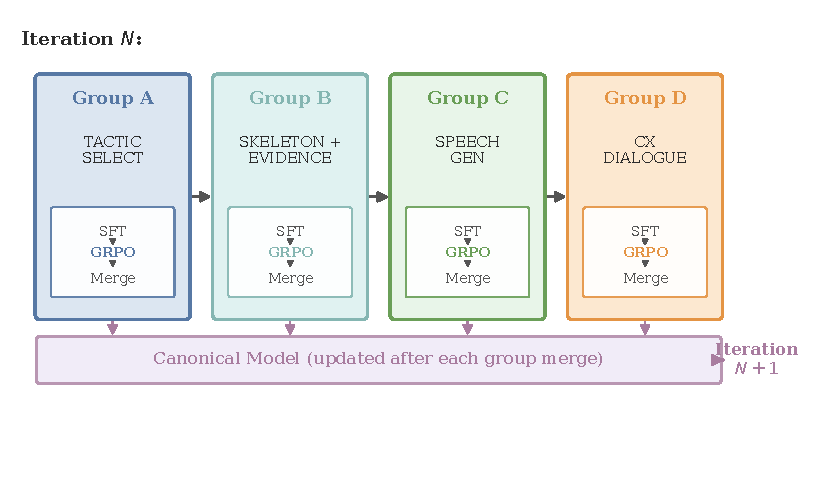
\includegraphics[width=\textwidth]{fig_grpo_pipeline.pdf}
\caption{Group-wise offline GRPO pipeline. Call types are partitioned into
four groups processed sequentially. Each group undergoes SFT on Opus
golden samples followed by offline GRPO with importance sampling. The
merged LoRA checkpoint from each group becomes the baseline for the next,
preventing cross-modality gradient interference.}
\label{fig:grpo_pipeline}
\end{figure*}

The debate pipeline produces four heterogeneous call types---tactic
selection, skeleton/evidence construction, speech generation, and
cross-examination dialogue---that differ dramatically in output length,
vocabulary, and evaluation criteria. Training a single GRPO objective
over all call types conflates these modalities and produces unstable
gradients. We instead partition calls into four groups (A--D), training
each sequentially with group-specific hyperparameters.

\subsection{Group Configurations}

\begin{table}[h]
\centering
\small
\begin{tabular}{lllrrrr}
\toprule
\textbf{Group} & \textbf{Call Types} & \textbf{Samples} & \textbf{Max Tok} & \textbf{Batch} & \textbf{Epochs} & \textbf{Val Acc} \\
\midrule
A & \textsc{Tactic\_Select} & 2,887 & 5,000 & 3--4 & 5 & 81.0\% \\
B & \textsc{Skeleton} + \textsc{Evidence} & 4,157 & 16,000 & 3 & 5 & 73.3\% \\
C & \textsc{Speech\_Generate} & 3,274 & 10,500 & 4 & 8 & 72.3\% \\
D & \textsc{CX\_Dialogue} & 5,003 & 7,000 & 4 & 4 & 87.5\% \\
\bottomrule
\end{tabular}
\caption{GRPO group configurations. Max tokens reflects the longest
completions in each group. Validation accuracy is measured on held-out
debates from the same iteration. Group~D achieves the highest validation
accuracy because CX responses have shorter, more constrained outputs.}
\label{tab:grpo_groups}
\end{table}

\paragraph{Why these groupings.}
Group~A (tactic selection) has the shortest outputs ($\sim$500--2,000
tokens) and the clearest reward signal: did the chosen tactic lead to
a high-scoring speech? Group~B (skeleton + evidence) is grouped because
skeleton structure and evidence selection are tightly coupled---a skeleton
designed around unavailable evidence fails at generation time. Group~C
(speech generation) has the longest outputs and the most subjective
evaluation, requiring more epochs to converge. Group~D (CX dialogue)
is isolated because dialogue has fundamentally different dynamics than
monologue (see Appendix~\ref{app:failure_modes} for the retry
degradation phenomenon specific to CX).

\subsection{SFT-GRPO Interleaving}

Each group follows a two-stage training protocol within each iteration:

\begin{enumerate}
\item \textbf{SFT on Opus golden samples.} Claude Opus generates
    high-quality reference outputs for each call type. The model is
    fine-tuned (SFT) on these samples to establish a strong behavioral
    prior, producing the SFT+ checkpoint.

\item \textbf{GRPO on preference pairs.} The SFT+ model generates
    $k{=}4$ trial outputs per call (with logprob capture). These trials
    are scored by the agentic judge (Appendix~\ref{app:agentic_judge}),
    producing preference pairs. GRPO then optimizes the model on these
    pairs with the group-specific hyperparameters.

\item \textbf{Merge to canonical.} The GRPO LoRA is merged into the
    canonical base model, which becomes the starting point for the next
    group.
\end{enumerate}

The sequential ordering (A $\rightarrow$ B $\rightarrow$ C $\rightarrow$ D)
is deliberate: tactic improvements (Group~A) propagate to skeleton
construction (Group~B), which propagates to speech generation (Group~C),
and finally dialogue (Group~D). Each group trains on top of the
improvements from all preceding groups within the same iteration.

\paragraph{Why SFT before GRPO.}
GRPO alone can only redistribute probability mass among behaviors the
model already exhibits. SFT on Opus golden samples introduces
\emph{new} high-quality behaviors (e.g., more sophisticated argument
structures, better evidence integration) that GRPO can then reinforce
through preference optimization. Without the SFT step, GRPO is
limited to choosing among the model's existing capabilities.

\subsection{Importance Sampling}

GRPO requires the log-probability of each response under the current
policy. In the offline setting, responses were generated by a
\emph{previous} policy checkpoint. We handle this via importance sampling:

\begin{enumerate}
\item \textbf{Logprob capture at generation time.} When the SFT+ model
    generates trial outputs, per-token log-probabilities are recorded
    alongside the text.

\item \textbf{Importance weight computation.} The GRPO loss uses
    $\pi_\theta(y|x) / \pi_{\text{ref}}(y|x)$ ratios, where
    $\pi_{\text{ref}}$ is the generating policy. Precomputed logprobs
    from step~1 serve as $\log \pi_{\text{ref}}$.

\item \textbf{Recomputation after merge.} After each group merge, the
    canonical model's policy has shifted. For subsequent groups, logprobs
    from earlier generations become stale. We recompute reference logprobs
    on a random 20\% subsample to estimate the KL divergence; if
    $D_\text{KL} > 0.5$, all logprobs for the affected group are
    recomputed before training.
\end{enumerate}

Stale logprobs were identified as a root cause of the Group~C regression
described in Appendix~\ref{app:experiment_details}: the importance
weights became extreme, producing unstable gradient updates.

\subsection{Advantage Normalization}

Standard GRPO normalizes advantages globally across the training batch.
This is problematic for debate because the difficulty of generating a
good response depends heavily on the strategic context: a tactic that
works well against one opponent strategy may fail against another.

We normalize advantages within \emph{context triplets}:
$(\text{our\_tactic}, \text{opponent\_tactic}, \text{opponent\_intent})$.
For each triplet, the advantage is:
\begin{equation}
A_i = r_i - \bar{r}_{\text{triplet}}
\end{equation}

\noindent where $\bar{r}_{\text{triplet}}$ is the mean reward across all
samples sharing the same context triplet. This ensures that a mediocre
response against a strong opponent tactic is not penalized as harshly as
the same response against a weak opponent tactic.

In practice, triplet normalization improved validation accuracy by 3--5
percentage points across all groups compared to global normalization,
with the largest improvement in Group~A (tactic selection), where
strategic context has the most direct influence on reward.

\subsection{Attention-Only LoRA}

During the Group~C regression investigation
(Appendix~\ref{app:experiment_details}), we discovered that
targeting all seven linear projection modules in the Qwen3-30B-A3B
architecture (q\_proj, k\_proj, v\_proj, o\_proj, gate\_proj, up\_proj,
down\_proj) produced 3.37 billion trainable parameters. This large
parameter count, combined with stale offline logprobs, caused
catastrophic divergence.

Restricting LoRA to attention projections only (q\_proj, k\_proj,
v\_proj, o\_proj) reduced trainable parameters to \textbf{53 million}---a
$\mathbf{64\times}$ reduction. Critically, this produced \textbf{no measurable
quality loss}: validation accuracy on Group~C was 72.3\% with
attention-only LoRA versus 72.1\% with the full 7-module LoRA (before
regression), while completely eliminating the instability.

\begin{table}[h]
\centering
\small
\begin{tabular}{lccc}
\toprule
\textbf{LoRA Config} & \textbf{Params} & \textbf{Val Acc} & \textbf{Stable?} \\
\midrule
Full (7 modules) & 3.37B & 72.1\% & No (regression at epoch 3) \\
Attention-only (4 modules) & 53M & 72.3\% & Yes (all 8 epochs) \\
\bottomrule
\end{tabular}
\caption{Comparison of LoRA configurations for Group~C GRPO training.
Attention-only LoRA achieves equivalent accuracy with $64\times$ fewer
parameters and complete training stability.}
\label{tab:lora_comparison}
\end{table}

We hypothesize that for Mixture-of-Experts architectures with offline
GRPO, the MLP expert layers (gate\_proj, up\_proj, down\_proj) are
particularly sensitive to importance weight noise because each expert
is activated sparsely---small perturbations to expert gating can
cascade into large output changes. Attention-only LoRA avoids this
failure mode entirely.

\subsection{Per-Group Training Dynamics}

\paragraph{Group A (Tactic Selection).}
Converges fastest (3 epochs to plateau). The primary learning signal is
tactic-outcome correlation: the model learns which macro-tactics succeed
against which opponent strategies. Validation accuracy reaches 81.0\%,
the highest among speech groups, reflecting the relatively constrained
output space.

\paragraph{Group B (Skeleton + Evidence).}
Requires the longest max token length (16,000) due to evidence card
formatting. The evidence verification penalty (Appendix~\ref{app:method_details})
provides a strong shaping signal: fabrication and hallucination receive
$2\times$ GRPO weight, driving the model toward verified citations early
in training.

\paragraph{Group C (Speech Generation).}
The most challenging group, requiring 8 epochs to converge. Early epochs
show improvement in argument structure; later epochs improve rhetorical
quality. The epsilon clipping parameter ($\varepsilon = 0.15$) is critical:
values above 0.20 risk the regression described in
Appendix~\ref{app:experiment_details}.

\paragraph{Group D (CX Dialogue).}
Achieves the highest validation accuracy (87.5\%) but the least
improvement over the SFT baseline, consistent with the finding in
Appendix~\ref{app:experiment_details} that CX dialogue resists
preference optimization. We attribute this to the interactive nature
of dialogue: CX quality depends as much on the opponent's responses
as on the model's own outputs, making the reward signal noisier.

\subsection{DeepSpeed ZeRO-3 Checkpoint Fix}

Training uses DeepSpeed ZeRO-3 across 8 GPUs, which shards model
parameters, gradients, and optimizer states across ranks. A subtle
issue arises at checkpoint time: na\"ively calling
\texttt{model.save\_pretrained()} saves only the local shard, producing
a corrupted checkpoint. The fix is to explicitly gather the full state
dictionary before saving:

\begin{enumerate}
\item Call \texttt{deepspeed.zero.GatheredParameters()} to reconstruct
    the full parameter tensors on rank~0.
\item Save the gathered state dict from rank~0 only.
\item Resume sharded training after the save completes.
\end{enumerate}

This issue is not specific to our pipeline but affects any ZeRO-3
training with LoRA adapters. We document it here because it caused
silent checkpoint corruption during early Group~B training runs,
producing models that loaded without error but generated degenerate
outputs.

\section{Trajectory and Reward Computation}
\label{app:trajectory}

This appendix details the full trajectory capture and reward computation
pipeline that connects debate execution to GRPO training signal.

\subsection{DebateTrajectory Structure}

Each debate produces a \texttt{DebateTrajectory} that records every
decision and its outcome:

\begin{table}[h]
\centering
\small
\begin{tabular}{lp{8cm}}
\toprule
\textbf{Field} & \textbf{Description} \\
\midrule
\texttt{speeches} & Ordered list of all speeches (AC, AC-CX, NC, NC-CX, 1AR, NR, 2AR) with full text and metadata \\
\texttt{aff\_turns} & List of \texttt{TurnRecord}s for the affirmative side \\
\texttt{neg\_turns} & List of \texttt{TurnRecord}s for the negative side \\
\texttt{judge\_scores} & Per-speech scores from all sub-judges (Appendix~\ref{app:agentic_judge}) \\
\texttt{branches} & List of \texttt{BranchState} records (Appendix~\ref{app:branching}) \\
\texttt{outcome} & Final debate result: winner, score differential, and judge reasoning \\
\texttt{debate\_id} & Unique identifier linking to the resolution and side assignments \\
\bottomrule
\end{tabular}
\caption{DebateTrajectory top-level fields.}
\label{tab:trajectory}
\end{table}

\subsection{TurnRecord}

Each turn within the trajectory captures the full decision context:

\begin{table}[h]
\centering
\small
\begin{tabular}{lp{8cm}}
\toprule
\textbf{Field} & \textbf{Description} \\
\midrule
\texttt{tactic\_selection} & The macro-tactic and micro-tactic sequence chosen for this turn \\
\texttt{opponent\_prediction} & The model's predicted opponent response (used for strategic planning) \\
\texttt{opponent\_ground\_truth} & The actual opponent response observed after the turn \\
\texttt{novelty\_bonus} & Reward bonus for using a novel tactic combination ($+0.05$ to $+0.15$) \\
\texttt{surprise\_bonus} & Reward bonus when the opponent's response differs significantly from prediction ($+0.05$ to $+0.10$), indicating the model explored territory not covered by the opponent model \\
\texttt{call\_records} & Per-call records for tactic, skeleton, evidence, and speech generation, each with logprobs \\
\bottomrule
\end{tabular}
\caption{TurnRecord fields capturing per-turn decision context.}
\label{tab:turn_record}
\end{table}

The \texttt{opponent\_prediction} and \texttt{opponent\_ground\_truth}
fields enable the surprise bonus: when the model's prediction diverges
substantially from reality, it indicates unexplored strategic territory
that may yield high-signal training examples.

\subsection{Reward Formula}

The per-turn reward combines four components reflecting different aspects
of debate quality:

\begin{equation}
r_{\text{combined}} = 0.25 \cdot r_{\text{selection}} + 0.35 \cdot r_{\text{execution}} + 0.25 \cdot r_{\text{quality}} + 0.15 \cdot r_{\text{novelty}}
\label{eq:combined_reward}
\end{equation}

\begin{table}[h]
\centering
\small
\begin{tabular}{lcp{6.5cm}}
\toprule
\textbf{Component} & \textbf{Weight} & \textbf{Source} \\
\midrule
$r_{\text{selection}}$ & 0.25 & Tactic appropriateness for the debate state; from Forensics module (Appendix~\ref{app:agentic_judge}) \\
$r_{\text{execution}}$ & 0.35 & Speech quality conditional on the tactic; composite of sub-judge scores \\
$r_{\text{quality}}$ & 0.25 & Speech-specific primary dimension score (Table~\ref{tab:speech_dimensions}) \\
$r_{\text{novelty}}$ & 0.15 & Novelty bonus $+$ surprise bonus from \texttt{TurnRecord} \\
\bottomrule
\end{tabular}
\caption{Per-turn reward components. Execution receives the highest weight
because it reflects the most direct measure of output quality.}
\label{tab:reward_components}
\end{table}

The final reward incorporates the debate outcome:
\begin{equation}
r_{\text{final}} = 0.7 \cdot r_{\text{combined}} + 0.3 \cdot r_{\text{win}}
\label{eq:final_reward}
\end{equation}

\noindent where $r_{\text{win}} \in \{0, 1\}$ is 1 if the model's side
won the debate and 0 otherwise. The 0.3 weight on the win bonus ensures
that outcome signal influences training without overwhelming the
fine-grained per-turn signal. Without the win bonus, the model could
learn to produce individually high-scoring speeches that collectively
lose the debate (e.g., strong individual arguments that fail to
cohere into a winning narrative).

\subsection{BackpropScorer Algorithm}

The BackpropScorer propagates debate-level outcomes back to individual
calls, producing causal attribution of which decisions most influenced
the result. This operates in four stages:

\paragraph{Stage 1: Outcome analysis.}
For each speech in the debate, compute its \emph{outcome contribution}
$c_s \in [-1.0, +1.0]$, estimating how much that speech contributed to
the final result. This is assessed by the scoring LLM, which receives
the full debate transcript and is asked: ``How much did [speech] contribute
to [side] winning/losing? Consider what would have changed if this speech
had been average rather than as-delivered.''

\paragraph{Stage 2: Branch counterfactual.}
For debates with branches (Appendix~\ref{app:branching}), identify the
divergence point and determine whether a winner shift occurred. If so,
the speeches at the divergence point receive amplified attribution:
their contribution scores are adjusted by the score differential between
the winning and losing branches.

\paragraph{Stage 3: Score adjustment.}
The final backpropagated score for each call is:
\begin{equation}
r_{\text{backprop}} = r_{\text{inline}} + c_s \cdot 0.2 + b_{\text{critical}} \cdot 0.15 + p_{\text{adj}}
\label{eq:backprop}
\end{equation}

\begin{table}[h]
\centering
\small
\begin{tabular}{lp{8cm}}
\toprule
\textbf{Term} & \textbf{Description} \\
\midrule
$r_{\text{inline}}$ & Original inline score from the sub-judges \\
$c_s \cdot 0.2$ & Outcome contribution scaled by 0.2 to prevent outcome signal from dominating \\
$b_{\text{critical}} \cdot 0.15$ & Critical call boost: $b_{\text{critical}} \in \{0, 1\}$ is 1 if Forensics identifies this call as a pivotal decision point \\
$p_{\text{adj}}$ & Pivotal adjustment from branch counterfactuals: ranges from $-0.5$ to $+0.5$ for winner-shifted decisions, 0 otherwise \\
\bottomrule
\end{tabular}
\caption{BackpropScorer adjustment terms.}
\label{tab:backprop_terms}
\end{table}

The multiplicative constants (0.2, 0.15) were tuned to keep
$r_{\text{backprop}}$ within approximately $\pm 0.3$ of
$r_{\text{inline}}$ for most calls, with larger adjustments reserved
for the small number of genuinely pivotal decisions (typically 2--3
per debate).

\paragraph{Stage 4: Reasoning preservation.}
The BackpropScorer generates a natural-language explanation for each
score adjustment, recording the causal chain from the call to the
debate outcome. These explanations are stored alongside the training
data for potential use in reasoning distillation---training the model
to internalize the judge's causal reasoning rather than just the
scalar reward.

\subsection{Group Baselines and Context Triplets}

As described in Appendix~\ref{app:grpo_groups}, GRPO advantages are
normalized within context triplets
$(\text{our\_tactic}, \text{opponent\_tactic}, \text{opponent\_intent})$.
The trajectory captures these triplets at each turn, enabling the
training pipeline to compute context-appropriate baselines.

\begin{table}[h]
\centering
\small
\begin{tabular}{lp{5cm}r}
\toprule
\textbf{Triplet Component} & \textbf{Source} & \textbf{Cardinality} \\
\midrule
Our tactic & \texttt{tactic\_selection} from TurnRecord & $\sim$25 macro-tactics \\
Opponent tactic & Inferred from opponent speech by the judge & $\sim$25 macro-tactics \\
Opponent intent & Classified as \textsc{Attack}, \textsc{Defend}, \textsc{Extend}, or \textsc{Probe} & 4 \\
\bottomrule
\end{tabular}
\caption{Context triplet components for advantage normalization. The
product space is large ($\sim$2,500 triplets) but most debates activate
only 15--30 distinct triplets, providing sufficient samples for
meaningful normalization.}
\label{tab:context_triplets}
\end{table}

\subsection{End-to-End Reward Flow}

Figure~\ref{fig:reward_flow} summarizes the complete reward computation
pipeline from debate execution to GRPO training signal.

\begin{figure}[h]
\centering
\small
\begin{tabular}{c}
\hline
\\[-0.5em]
\textbf{Debate Execution} \\
$\downarrow$ \\
\texttt{DebateTrajectory} (speeches, turns, branches) \\
$\downarrow$ \\
\textbf{Layer 1: Inline Scoring} \\
4 sub-judges $\times$ speech-specific dimensions $\rightarrow$ $r_{\text{inline}}$ \\
$\downarrow$ \\
\textbf{Layer 2: Outcome Backpropagation} \\
$r_{\text{inline}} + \text{outcome contribution} + \text{critical boost} + \text{branch adjustment}$ $\rightarrow$ $r_{\text{backprop}}$ \\
$\downarrow$ \\
\textbf{Layer 3: Meta-Debate Calibration} \\
3-model panel $+$ bias detection $+$ judge-the-judge filtering \\
$\downarrow$ \\
\textbf{Reward Assembly} \\
$r_{\text{final}} = 0.7 \cdot r_{\text{combined}} + 0.3 \cdot r_{\text{win}}$ \\
$\downarrow$ \\
\textbf{Triplet Normalization} \\
$A_i = r_i - \bar{r}_{(\text{our\_tactic}, \text{opp\_tactic}, \text{opp\_intent})}$ \\
$\downarrow$ \\
\textbf{GRPO Training} (Group A $\rightarrow$ B $\rightarrow$ C $\rightarrow$ D) \\
\\[-0.5em]
\hline
\end{tabular}
\caption{End-to-end reward flow from debate execution to GRPO training.
Each layer adds finer-grained signal: inline scoring evaluates individual
speeches, backpropagation attributes outcomes to decisions, and
meta-debate calibration removes judge bias.}
\label{fig:reward_flow}
\end{figure}

\section{Debate Generation Pipeline Details}
\label{app:pipeline}

This appendix expands Section~\ref{sec:pipeline}. The pipeline is shared
identically between baseline and experimental runs; all quality differences
reported in the main body therefore come from the speech generation model
and training procedure, not from asymmetric preparation.

\subsection{Belief Tree Structure}

From a resolution $R$, the pipeline constructs a typed belief tree in three
passes.

\paragraph{Values.}
A DSPy \textsc{ValueExtractor} module generates 4 topic-specific values,
2 per side, phrased as terminal goods the side should be understood to
defend (e.g., \emph{economic mobility}, \emph{institutional trust}).
Values are the roots of the belief tree.

\paragraph{Beliefs.}
A \textsc{BeliefGenerator} expands each value into 2 child beliefs per
side, then refines each to depth-2, yielding approximately 32 beliefs
total and 16 arguments per side. Each belief $b$ carries a Bayesian
credence $c(b)\in[0,1]$; the prior is set by the generator and is later
updated as posteriors conditioned on speeches delivered.

\paragraph{Arguments.}
Leaf beliefs are instantiated as typed arguments drawn from standard
debate theory: \textsc{uniqueness}, \textsc{link}, \textsc{impact},
\textsc{solvency}, and \textsc{turn}. Typing is important: it gives the
downstream speech stages structured slots (e.g., an impact argument must
identify magnitude, timeframe, probability), and it allows the hierarchical
reward (Section~\ref{sec:reward_hierarchy}) to reason about the debate at
the level of argument roles rather than raw sentences.

\subsection{Research Pipeline: v1 vs.\ v2}

\paragraph{v1 (9 LLM calls per hop).}
The original research agent made separate LLM calls for: query
formulation, query rewriting, relevance filtering, per-document
summarization, per-sentence judgement, selection ranking, card tagging,
citation extraction, and hop termination. Typical claims took 3--4 hops,
burning $\sim$30 calls per claim and dominating preparation cost.

\paragraph{v2 (2 LLM calls per hop, consolidated).}
The consolidated loop per claim is:
\begin{enumerate}
    \item \textbf{Query generation (LLM call 1):} A single structured call
    emits $k$ retrieval queries plus termination heuristics.
    \item \textbf{Parallel retrieval:} Weaviate (dense) and Tavily (web)
    run in parallel on each query.
    \item \textbf{Deterministic processing:} Text is cleaned, chunked into
    sentences, and scored with hybrid
    $s = 0.7\cdot \cos(\mathbf{q},\mathbf{s}) + 0.3\cdot\mathrm{BM25}(q,s)$.
    Top sentences are expanded into windows to preserve local context.
    \item \textbf{Selection (LLM call 2):} A single structured call
    consumes the candidate windows and emits the final evidence card via
    Pydantic validation, including bolded selections and sentence IDs.
\end{enumerate}
Most claims terminate after one hop. Total calls per claim drop from
$\sim$30 to $\sim$2--4, a 10$\times$ reduction that is what makes the
downstream branching tree (Section~\ref{sec:branching}) economically
feasible.

\subsection{Evidence Card Schema}

Each card is a Pydantic record with the following fields:
\begin{itemize}
    \item \texttt{tag} --- one-line argumentative claim.
    \item \texttt{cite}, \texttt{fullcite} --- short and full citations.
    \item \texttt{full\_text} --- the complete retrieved passage.
    \item \texttt{card} --- the passage with \textbf{bolded} sentences
    indicating selected material.
    \item \texttt{selected\_texts} --- list of selected sentences as
    strings.
    \item \texttt{selected\_sentence\_ids} --- indices into
    \texttt{full\_text}, the \emph{only} handle the speech generator can
    cite.
    \item \texttt{window\_ranges} --- windows around each selection used
    for context.
    \item \texttt{source\_url} --- retrieval source for audit.
    \item \texttt{relevance\_score} --- retrieval score used by sorting.
\end{itemize}
Because downstream speech generation cites by \texttt{selected\_sentence\_id}
only, the quotation text is mechanically assembled from \texttt{full\_text}
and cannot be fabricated by the model. This is the structural property that
makes evidence verification in Section~\ref{sec:reward_hierarchy} a
sentence-ID check rather than a natural-language fidelity judgment.

\subsection{Perspective Building}

Given the completed belief tree, a \textsc{PerspectiveBuilder} compiles
side-specific prompt contexts:
\begin{itemize}
    \item \textbf{Constructives} receive a pruned depth-1 view: 2 of the
    4 root beliefs for the side, chosen to cover complementary ground.
    This forces the constructive speech to commit to a narrow thesis
    rather than diffuse across all available arguments.
    \item \textbf{Rebuttals} receive the full sub-belief tree in SEAM
    form (Setup, Evidence, Analysis, Move), which aligns naturally with
    rebuttal block structure in competitive debate.
    \item \textbf{CX} receives the opponent's most recent
    constructive along with attackable beliefs.
\end{itemize}
Different branches of the debate tree (Section~\ref{sec:branching}) are
seeded with different D1 belief combinations, producing natural debate
diversity without any hand-written prompts or per-topic tuning.

\subsection{Why Automation Matters}

\paragraph{Reproducibility.}
Every piece of training data is reproducible from the original resolution
plus the research index snapshot: there is no human-curated brief, no
pre-written argument, no case file. This matters for scientific validity;
it also matters for operational robustness when we replay or audit
training runs.

\paragraph{Scale.}
The pipeline runs end-to-end on a resolution in minutes, making tournament
generation (68 debates) and training-scale generation (thousands of
debates) feasible on a small budget ($\sim$\$750--1{,}000 total;
Appendix~\ref{app:costs}).

\paragraph{Baseline/experimental comparability.}
The same pipeline produces the inputs for both the base Qwen3-30B-A3B and
all trained checkpoints. A difference in downstream win rate therefore
cannot be attributed to a richer prep stage, a better research index, or
stronger evidence --- the substrate is identical, so the delta isolates the
generation model. This is a property we rely on for the tournament
analysis in Section~\ref{sec:analysis}.

\paragraph{Ablation surface.}
Because the pipeline is structured rather than monolithic, components can
be ablated independently: belief tree depth, research-hop limits, SEAM
structure, and the four-stage decomposition itself. Each is a natural
axis of ablation and a natural training target, independent of the
specific model being trained.


\end{document}
